% !TEX root = ./thesis.tex
\graphicspath{{./vega-arch/figures/}}
\chapter{A Streaming Dataflow Architecture}
\label{sec:vg:arch}

\begin{figure}[h!]
  \vspace{-40pt}
  \centering
  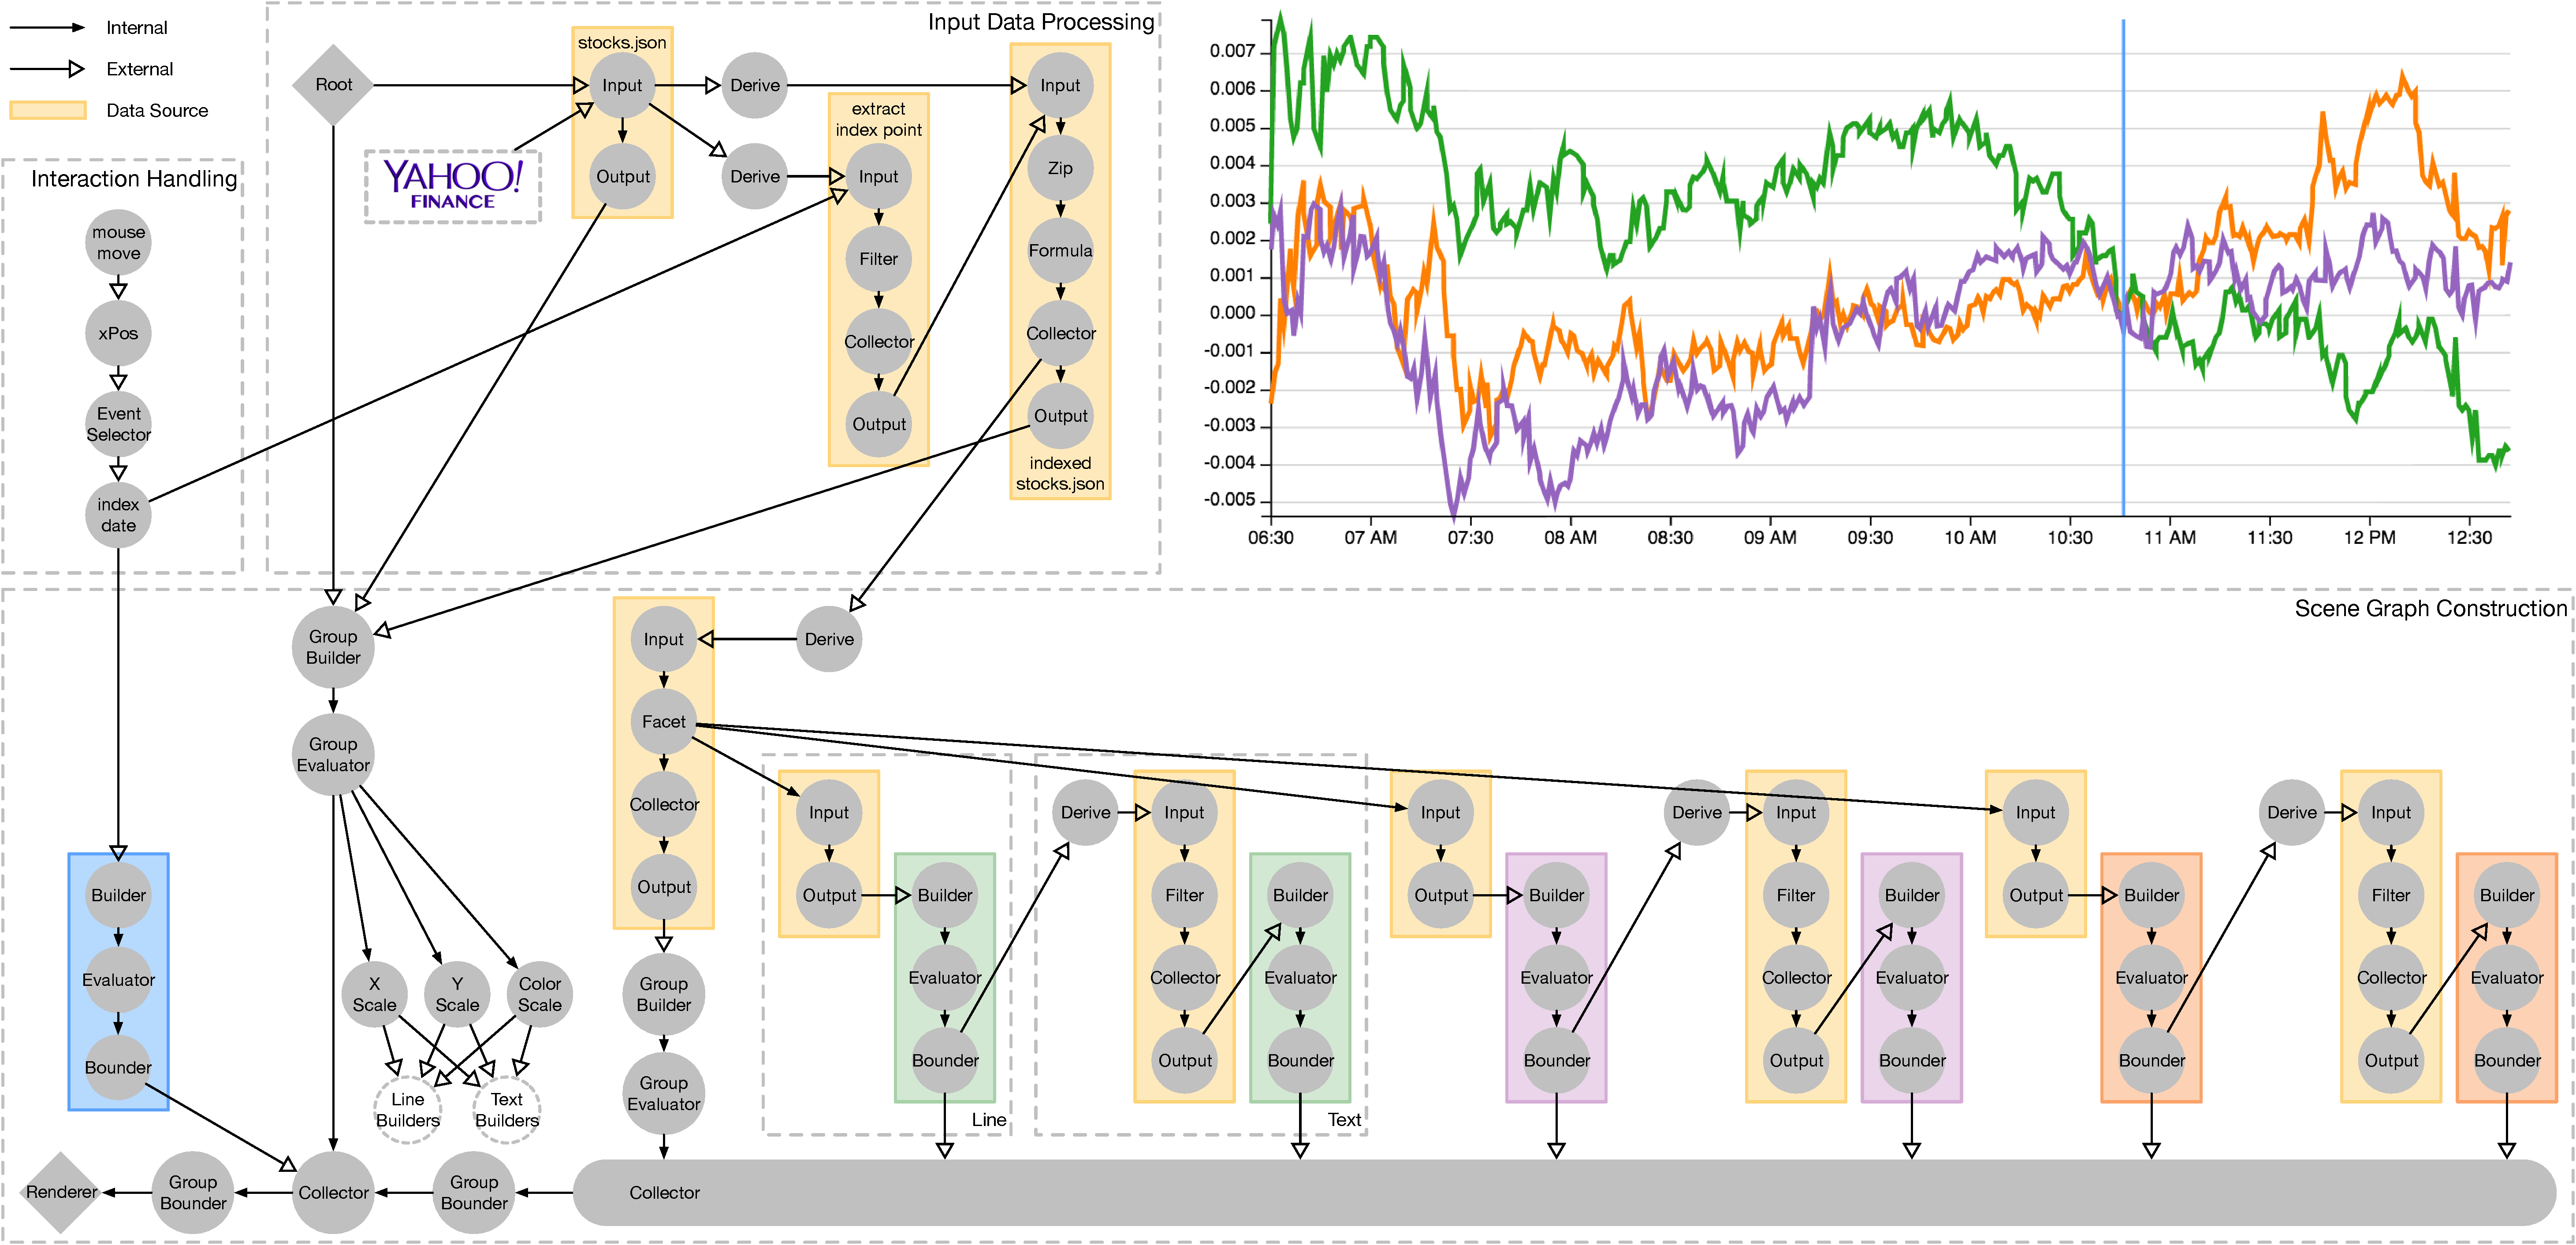
\includegraphics[width=\columnwidth]{teaser}
  \caption{The Reactive Vega dataflow graph created for a interactive index
  chart of streaming financial data. As streaming data arrives from the Yahoo!
  Finance API, or as a user moves their mouse pointer across the chart, an
  update cycle propagates through the graph and triggers an efficient update and
  re-render of the visualization.}
  \label{fig:vg:teaser}
\end{figure}

While the previous chapter describes the design of Reactive Vega's declarative
interaction design model, we now turn to the system architecture needed to
support it. Our architecture design is motivated by four primary goals:

\begin{enumerate}
  \item \textbf{A Unified Data Model}. Existing reactive visualization
toolkits (e.g., Model.js~\cite{kelleher:modeljs}) feature fragmented
architectures where only interaction events are modeled as time-varying. Other
input datasets remain static and batch-processed. This artificial disconnect
restricts expressivity and can result in wasteful computation. For example,
interaction events that manipulate only a subset of input tuples may trigger
recomputation over the entire dataset. In contrast, Reactive Vega features a
unified data model in which input data, scene graph elements, and interaction
events are all treated as first-class streaming data sources.

  \item \textbf{Streaming Relational Data}. Modeling input relational data with
Event-Driven Functional Reactive Programming (E-FRP)~\cite{wan:efrp} semantics
alone does not supply sufficient granularity for targeted recomputation. As
E-FRP semantics consider only time-varying scalar values, operators would
observe an entire relation as having changed and so would need to reprocess all
tuples. Instead, Reactive Vega integrates techniques from streaming
databases~\cite{abadi:borealis, abadi:aurora, arasu:stream, avnur:eddies,
chandrasekaran:telegraphcq} alongside E-FRP, including tracking state at the
tuple-level and only propagating modified tuples through the dataflow graph.

  \item \textbf{Streaming Nested Data}. Interactive visualizations, particularly
those involving small multiples, often require hierarchical structures.
Processing such data poses an additional challenge not faced by prior reactive
or streaming database systems. To support streaming nested data, Reactive Vega's
dataflow graph rewrites itself in a data-driven fashion at runtime: new branches
are extended, or existing branches pruned, in response to observed hierarchies.
Each dataflow branch models its corresponding part of the hierarchy as a
standard relation, enabling operators to remain agnostic to higher-level
structure.

  \item \textbf{Interactive Performance}. Reactive Vega performs both compile-
and run-time optimizations to increase throughput and reduce memory footprint,
including tracking metadata to prune unnecessary computation, and optimizing
scheduling by inlining linear chains of operators. We conduct benchmark
studies of streaming and interactive visualizations and find that Reactive
Vega meets or exceeds the performance of both D3 and the original, unreactive
Vega system.
\end{enumerate}

Reactive Vega is implemented in the JavaScript programming language, and is
intended to run either in a web browser or server-side using Node.js. By
default, Reactive Vega renders to an HTML5 Canvas element; however, it also
supports Scalable Vector Graphics (SVG) and server-side image rendering.

% !TEX root = ../thesis.tex
\section{The Dataflow Graph Design}
\label{sec:vg:dataflow}

Operators in Reactive Vega's dataflow graph are instantiated and connected by
its \emph{parser}, which traverses a declarative specification containing
definitions for input datasets, visual encoding rules, and interaction
primitives as described in~\cref{sec:vg:lang}. When data tuples are observed, or
when interaction events occur, they are propagated (or ``\emph{pulsed}'')
through the graph with each operator being evaluated in turn. Propagation ends
at the graph's sole sink: the renderer.

\subsection{Data, Interaction, and Scene Graph Operators}

Reactive Vega's dataflow operators fall into one of three categories: input data
processing, interaction handling, or scene graph construction.

\subsubsection{Processing Input Data}

Reactive Vega parses each dataset definition and constructs a corresponding
branch in the dataflow graph. These branches comprise input and output nodes
connected by a pipeline of data transformation operators. Input nodes receive
raw tuples as a linear stream (tree and graph structures are supported via
parent-child or neighbor pointers, respectively). Upon data source updates,
tuples are flagged as either \emph{added}, \emph{modified}, or \emph{removed},
and each tuple is given a unique identifier. Data transformation operators use
this metadata to perform targeted computation and, in the process, may derive
new tuples from existing ones. Derived tuples retain access to their ``parent''
via prototypal inheritance\,---\,operators need not propagate unrelated upstream
changes.

Some operators require additional inspection of tuple state. Consider an
aggregate operator that calculates running statistics over a dataset (e.g.,
mean and variance). When the operator observes added or removed tuples, the
statistics can be updated based on the current tuple values. With modified
tuples, the previous value must be subtracted from the calculation and the new
value added. Correspondingly, tuples include a \texttt{previous} property.
Writes to a tuple attribute are done through a setter function that copies
current values to the \texttt{previous} object.

\subsubsection{Handling Interaction}

Reactive Vega instantiates an event listener node in the dataflow graph for each
low-level event type required by the visualization (e.g., \texttt{mousedown} or
\texttt{touchstart}). These nodes are directly connected to dependent signals as
specified by event selectors~\cite{satyanarayan:declarative}. In the case of
ordered selectors (e.g., a ``drag'' event specified by \texttt{[mousedown,
mouseup] > mousemove}), each constituent event is connected to an automatically
created anonymous signal; an additional anonymous signal connects them to serve
as a gatekeeper, and only propagates the final signal value when appropriate.
Individual signals can be dependent on multiple event nodes and/or other
signals, and value propagation follows E-FRP's two-phase update~\cite{wan:efrp}
as described in~\secref{sec:propagation}.

\subsubsection{Constructing the Scene Graph}

\begin{figure}[h!]
  \centering
  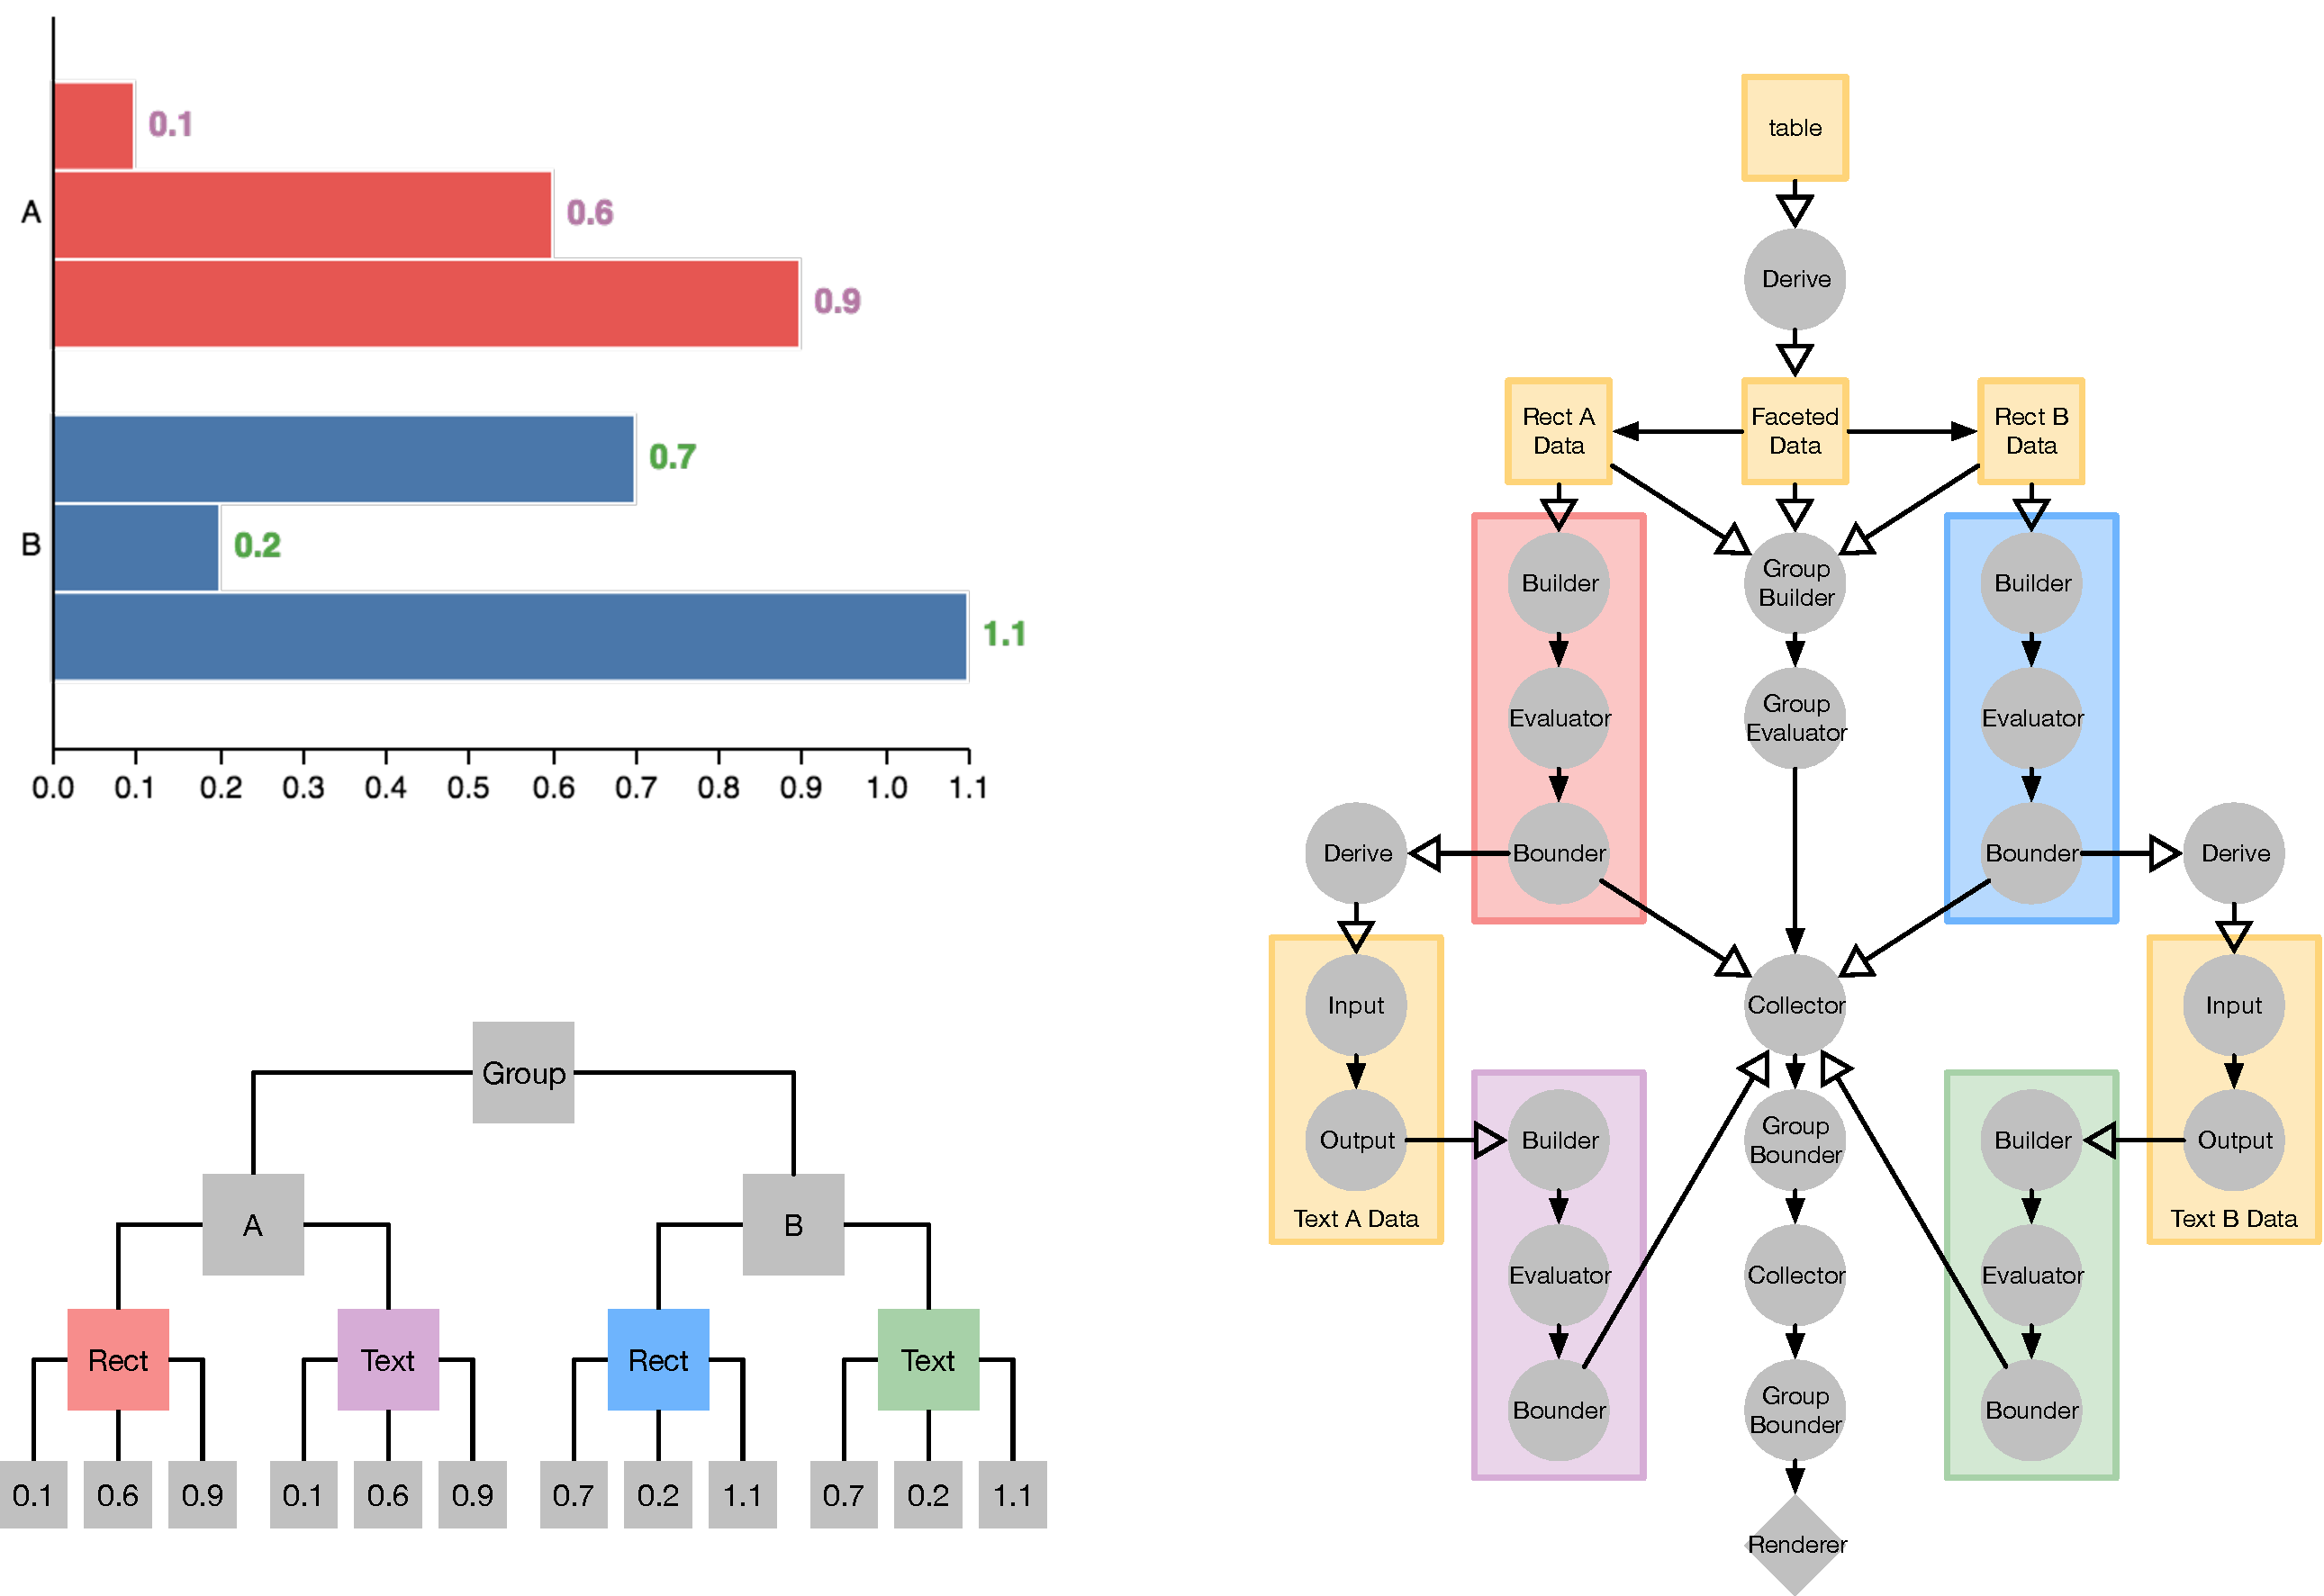
\includegraphics[width=0.9\columnwidth]{groupedBar}
  \caption{A grouped bar chart (top), with the underlying scene graph (bottom),
  and corresponding portion of the dataflow graph (right).}
  \label{fig:vg:groupedBar}
\end{figure}

\begin{figure}[h!]
  \centering
  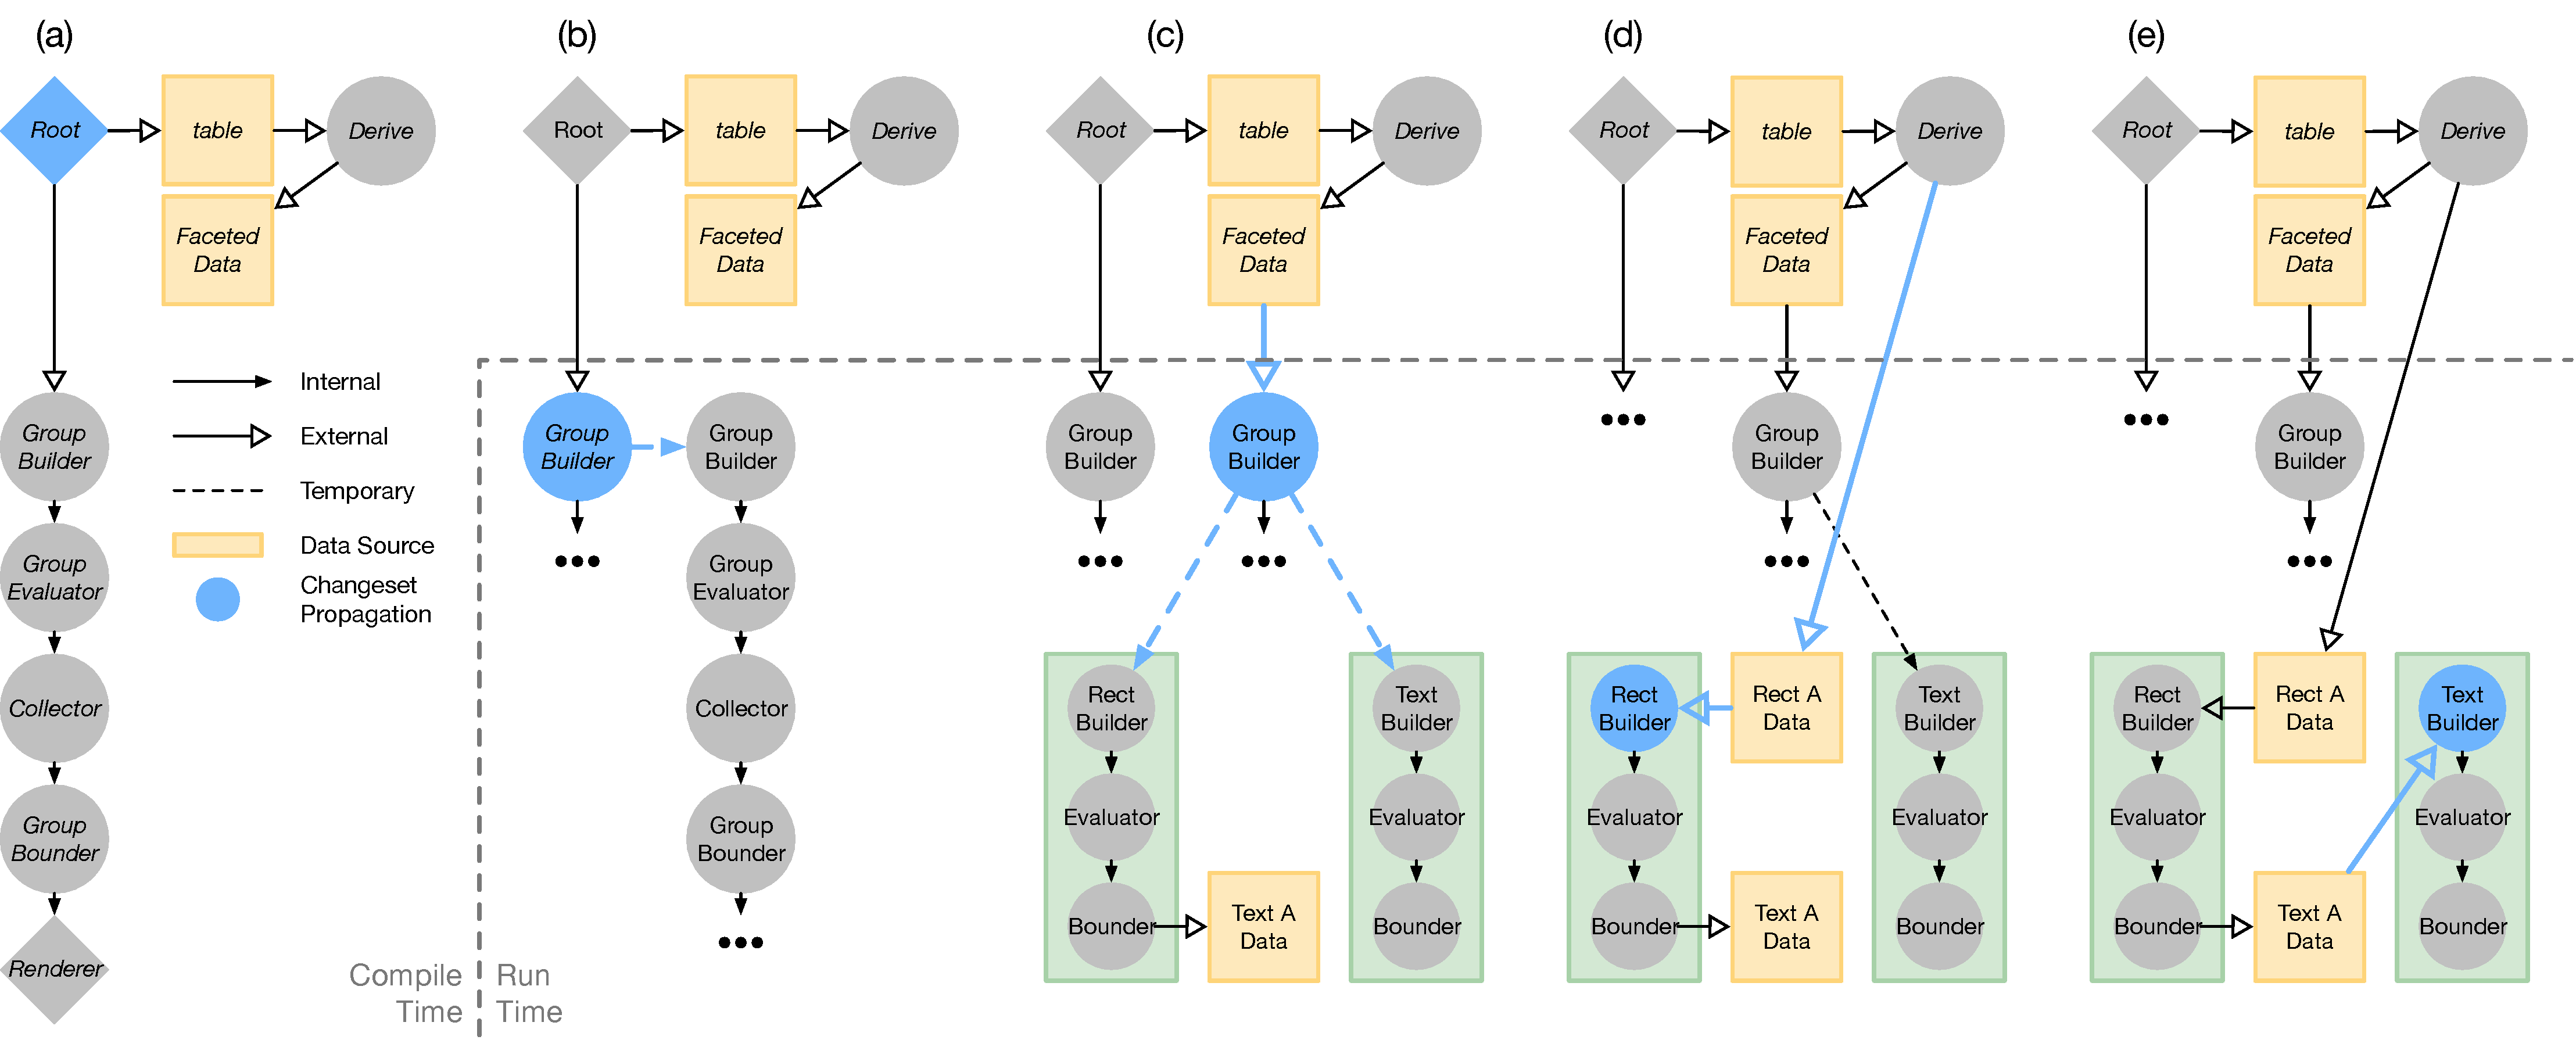
\includegraphics[width=\columnwidth]{scenegraph}
  \caption{Dataflow operators responsible for scene graph construction are
dynamically instantiated at run-time, a process that results in the graph seen
in Fig.~\ref{fig:vg:groupedBar}. (a) At compile-time, a branch corresponding  to
the root scene graph node is instantiated. (b-c) As the changeset (in blue)
propagates through nodes, group-mark builders instantiate builders for their
children. Parent and child builders are temporarily connected (dotted lines) to
ensure children are built in the same timecycle. (d-e) When the changeset
propagates to the children, the temporary connection is replaced with a
connection to the mark's backing data source (also in blue).}
  \label{fig:vg:scenegraph}
\end{figure}

To construct the scene graph, Reactive Vega follows a process akin to the
Protovis bind-build-evaluate pipeline~\cite{heer:protovisjava}. When a
declarative specification is parsed, Reactive Vega traverses the mark hierarchy
to \emph{bind} property definitions: property sets are compiled into encoding
functions and stored with the specification. At run-time, \emph{build} and
\emph{evaluate} operators are created for each bound mark. The build operator
performs a data join~\cite{bostock:d3} to generate one scene graph element (or
``mark'') per tuple in the backing dataset, and the evaluate operator runs the
appropriate encoding functions. A downstream \emph{bounds} operator calculates
the bounding boxes of generated marks. For a nested scene graph to be rendered
correctly, the order of operations is critical: parent marks must be built and
encoded before their children, but the bounds of the children must be calculated
before their parents. The resultant scene graph exhibits an alternating
structure, with individual mark elements grouped under a sentinel mark
specification node. \Cref{fig:vg:scenegraph} illustrates this process for a
grouped bar chart.

Scene graph elements are also modeled as data tuples and can serve as the input
data for downstream visual encoding primitives. This establishes a
\emph{reactive geometry} that accelerates common layout tasks, such as label
positioning, and expands the expressiveness of the specification language. As
marks can be run through subsequent data transformations, higher-level layout
algorithms (e.g., those that require a pre-computed initial
layout~\cite{flexbox}) are now supported in a fully declarative fashion.

\subsection{Changesets and Materialization}

All data does not flow through the system at all times. Instead, operators
receive and transmit \emph{changesets}. A changeset consists of tuples that have
been observed, new signal values, and updates to other dependencies that have
transpired since the last render event. The propagation of a changeset begins in
response to streaming tuples or user interaction. The corresponding input node
creates a fresh changeset, and populates it with the detected update. As the
changeset flows through the graph, operators use it to perform targeted
recomputation, and may augment it in a variety of ways. For example, a
\texttt{Filter} operator might remove tuples from a changeset if they do not
meet the filter predicate, or may mark modified tuples as \texttt{added} if they
previously had been filtered. A Cartesian product operator, on the other hand,
would replace all incoming tuples with the cross-product with another data
stream.

While changesets only include updated data, some operators require a complete
dataset. For example, a windowed-join requires access to all tuples in the
current windows of the joined data sources. For such scenarios, special
\emph{collector} operators (akin to \emph{views}~\cite{abadi:aurora} or
\emph{synopses}~\cite{arasu:stream} in streaming databases) exist to
materialize the data currently in a branch. In order to mitigate the
associated time and memory expenses, Reactive Vega automatically shares
collectors between dependent operators. Upon instatiation, such operators must
be annotated as requiring a collector; at run-time they can then request a
complete dataset from the dataflow graph scheduler.

Finally, if animated transitions are specified, a changeset contains an
interpolation queue to which mark evaluators add generated mark instances; the
interpolators are then run when the changeset is evaluated by the renderer.

\subsection{Coordinating Changeset Propagation}
\label{sec:propagation}

A centralized dataflow graph scheduler is responsible for dispatching changesets
to appropriate operators. The scheduler ensures that changeset propagation
occurs in topological order so that an operator is only evaluated after all of
its dependencies are up-to-date. This schedule prevents wasteful intermediary
computation or momentary inconsistencies, known as
\emph{glitches}~\cite{cooper:embedding}. Centralizing this responsibility,
rather than delegating it to operators, enables more aggressive pruning of
unnecessary computation as described in~\secref{sec:pruning}. The scheduler has
access to the full graph structure and, thus, more insight into the state of
individual operators and propagation progress.

When an interaction event occurs, however, an initial non-topological update of
signals is performed. Dependent signals are reevaluated according to their
specification order. As a result, signals may use prior computed values of their
dependencies, which will subsequently be updated. This process mimics E-FRP's
two-phase update~\cite{wan:efrp}, and is necessary to enable expressive signal
composition. Once all necessary signals have been reevaluated, a changeset with
the new signal values is sent to the scheduler for propagation to the rest of
the dataflow graph.

\subsection{Pushing Internal and Pulling External Changesets}

Two types of edges connect operators in the dataflow graph. The first connects
operators that work with the same data; for example a pipeline of data
transformation operators for the same data source, or a mark's build and
evaluate operators. Changesets are pushed along these edges, and operators
use and augment them directly.

The second type of edge connects operators with external dependencies such as
other data sources, signals, and scale functions. As these edges connect
disparate data spaces, they cannot directly connect operators with their
dependencies. To do otherwise would result in operators performing computation
over mismatched data types. Instead, external dependencies are connected to
their dependents' nearest upstream \texttt{Collector} node, and changesets that
flow along these edges are flagged as \emph{reflow changesets}. When a
\texttt{Collector} receives a reflow changeset, it propagates its tuples
forward, flagging them as modified. The dependents now receive correct input
data and request the latest values of their dependencies from the scheduler.

The only exception to this pattern is when signals rely on other signals.
Reflow changesets still flow along these edges but, as they operate in scalar
data space, they are not mediated by \texttt{Collectors}.

This hybrid push/pull system enables a complex web of interdependent operators
while reducing the complexity of individual elements. For example, regardless of
whether a signal parameterizes data transforms or visual encoding primitives, it
simply needs to output a reflow changeset. Without such a system in place, the
signal would instead have to construct a different changeset for each dependency
edge it was a part of, and determine the correct dataset to supply. \Cref
{fig:vg:teaser,} use
filled and unfilled arrows for internal and external
connections, respectively.

\subsection{Dynamically Restructuring the Graph}

To support streaming nested data structures, operators can dynamically
restructure the graph at runtime by extending new branches, or pruning
existing ones, based on observed data. These dataflow branches model their
corresponding hierarchies as standard relations, thereby enabling subsequent
operators to remain agnostic to higher-level structure. For example, a
\texttt{Facet} operator partitions tuples by key fields; each partition then
propagates down a unique, dynamically-constructed dataflow branch, which can
include other operators such as \texttt{Filter} or \texttt{Sort}.

In order to maintain interactive performance, new branches are queued for
evaluation as part of the same propagation in which they were created. To
ensure changeset propagation continues to occur in topological order,
operators are given a \emph{rank} upon instantiation to uniquely identify
their place in the ordering. When new edges are added to the dataflow graph,
the ranks are updated such that an operator's rank is always greater than
those of its dependencies. When the scheduler queues operators for
propagation, it also stores the ranks it observes. Before propagating a
changeset to an operator, the scheduler compares the operator's current rank
to the stored rank. If the ranks match, the operator is evaluated; if the
ranks do not match, the graph was restructured and the scheduler requeues the
operator.

The most common source of restructuring operations are scene graph operators, as
building a nested scene graph is entirely data-driven. Dataflow branches for
child marks (consisting of build-evaluate-bound chains) cannot be instantiated
until the parent mark instances have been generated. As a result, only a single
branch, corresponding to the root node of the scene graph, is constructed at
compile-time. As data streams through the graph, or as interaction events occur,
additional branches are created to build and encode corresponding nested marks.
To ensure their marks are rendered in the same propagation cycle, new branches
are temporarily connected to their parents. These connections are subsequently
removed so that children marks will only be rebuilt and re-encoded when their
backing data source updates. Figure~\ref{fig:vg:scenegraph} provides a
step-by-step illustration of how scene graph operators are constructed during a
propagation cycle for the grouped bar chart in Figure~\ref{fig:vg:groupedBar}.
% !TEX root = ../thesis.tex
\section{Performance Optimizations}
\label{sec:vg:optimizations}

Declarative language runtimes can transparently optimize
performance~\cite{heer:protovisjava} and Reactive Vega uses several strategies
to increase throughput and reduce memory usage. In this section, we describe
these strategies and evaluate their effect through benchmark studies. Each
benchmark was run with datasets sized at N = 100, 1,000, 10,000, and 100,000
tuples. For ecological validity, benchmarks were run with Google Chrome 42
(64-bit) and, to prevent confounds with browser-based just-in-time (JIT)
optimizations, each iteration was run in a fresh instance. All tests were
conducted on a MacBook Pro system running Mac OS X 10.10.2, with a quad-core
2.5GHz Intel Core i7 processor and 16GB of 1600 MHz DDR3 RAM.

\subsection{On-Demand Tuple Revision Tracking}

\begin{figure}[h!]
  \centering
  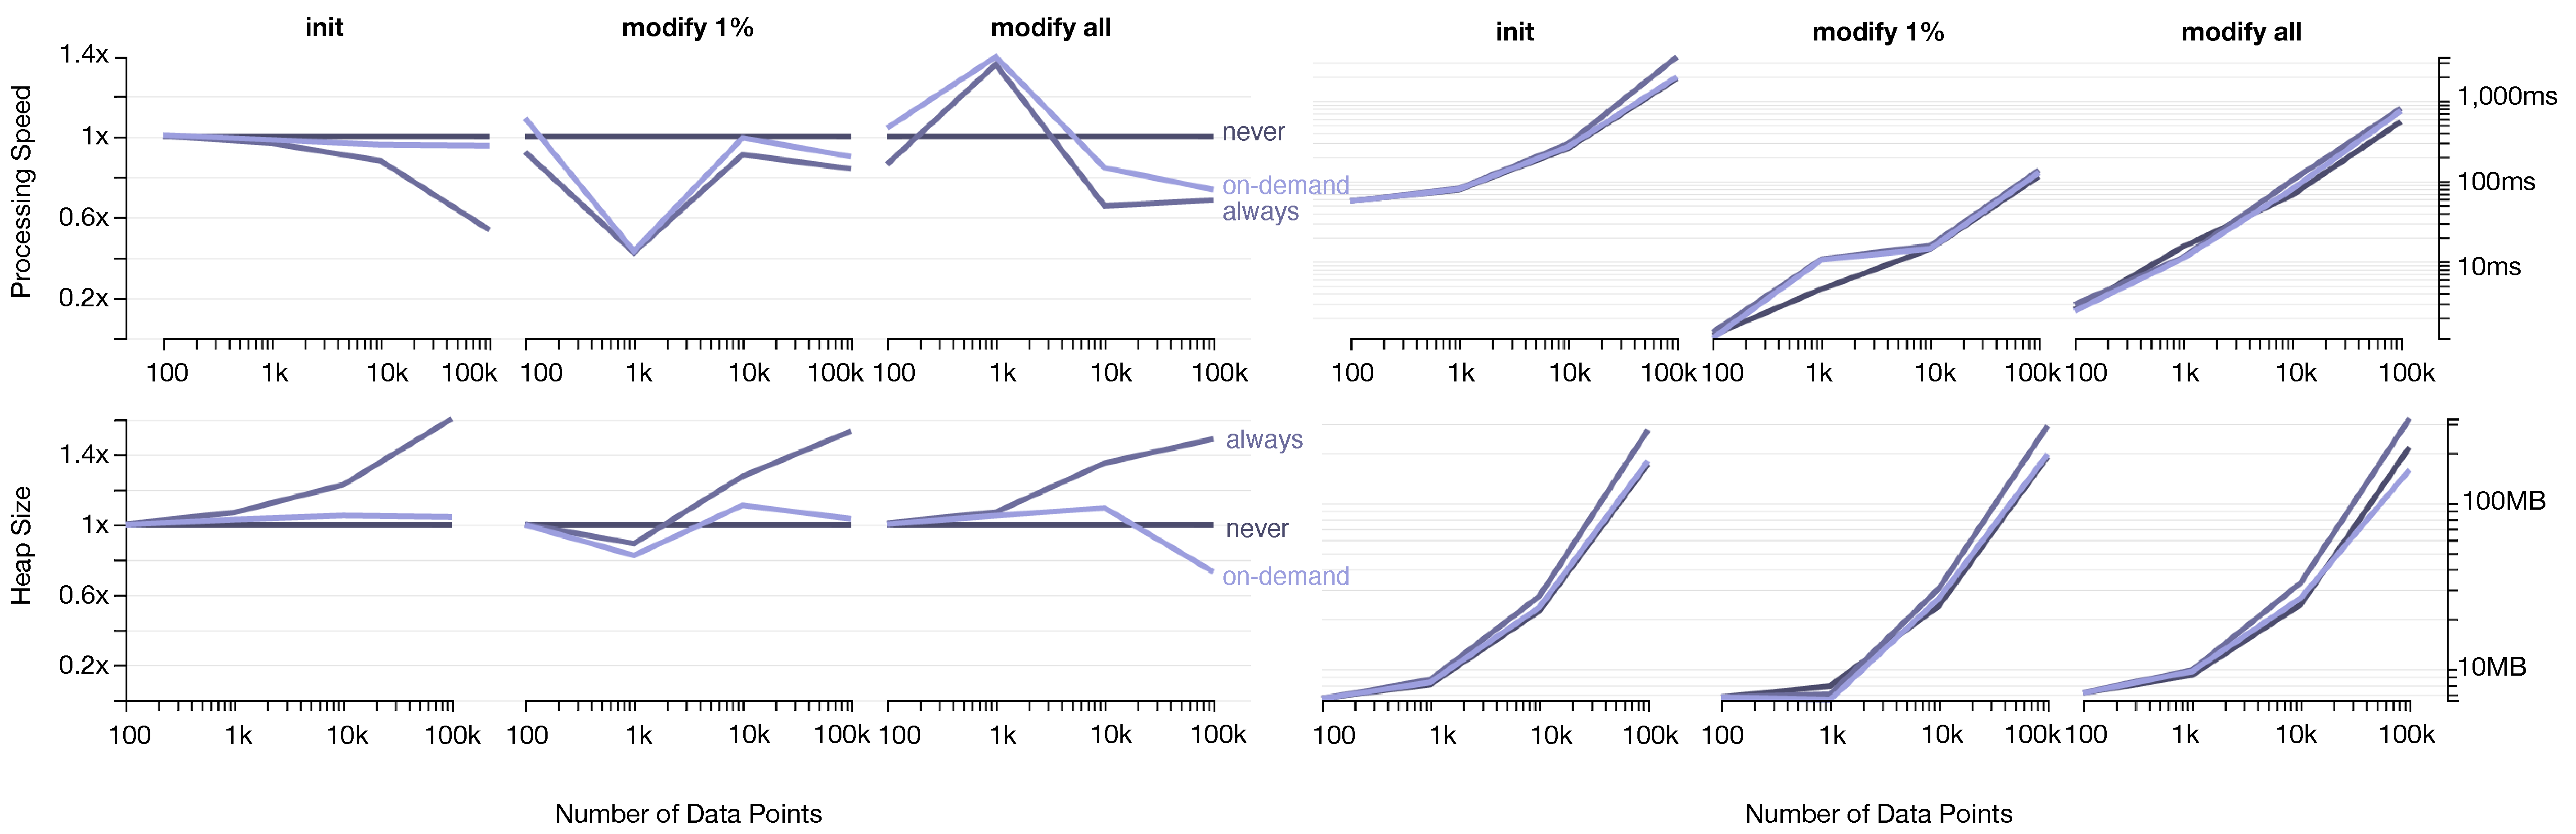
\includegraphics[width=\columnwidth]{prev-lines.pdf}
  \caption{Effects of tuple revision optimizations on average
processing speed (top) and memory footprint (bottom). Left-hand figures show
relative changes using no-tracking as a baseline (closer to 1.0 are better),
and right-hand figures show the absolute values on a log$_{10}$ scale
(lower is better).}
  \label{fig:vg:prev_benchmark}
\end{figure}

Some operators (e.g., statistical aggregates) require both a tuple's current and
previous values. Tracking prior values can affect both running time and memory
consumption. One strategy to minimize this cost is to track tuple revisions only
when necessary. Operators must declare their need for prior values. Then, when
tuples are ingested, their previous values are only tracked if the scheduler
determines that they will flow through an operator that requires revision
tracking.

We ran a benchmark comparing three conditions: always track revisions, never
track revisions, and on-demand tracking. Although the ``never'' condition
produces incorrect results, it provides a lower-bound for performance. We
measured the system's throughput as well as memory allocated when initializing a
scatterplot specification, and after modifying either 1\% or 100\% of input
tuples. The scatterplot features two symbol marks fed by two distinct dataflows,
\texttt{A} and \texttt{B}. Both branches ingest the same set of tuples, and
include operators that derive new attributes. However, \texttt{B} includes
additional aggregation operators that require revision tracking.

The results are shown in Figure~\ref{fig:vg:prev_benchmark}, with the effects of
revision tracking most salient at larger dataset sizes. Always tracking
revisions can require 20-40\% more memory, and can take up to 50\% longer to
initialize a visualization due to object instantiation overhead for storing
previous values. Our on-demand strategy effectively reduces these costs,
requiring only 5-10\% more memory and taking 5\% longer to initialize than the
``never'' condition.

\subsection{Pruning Unnecessary Recomputation}
\label{sec:pruning}

\begin{figure}[h!]
  \centering
  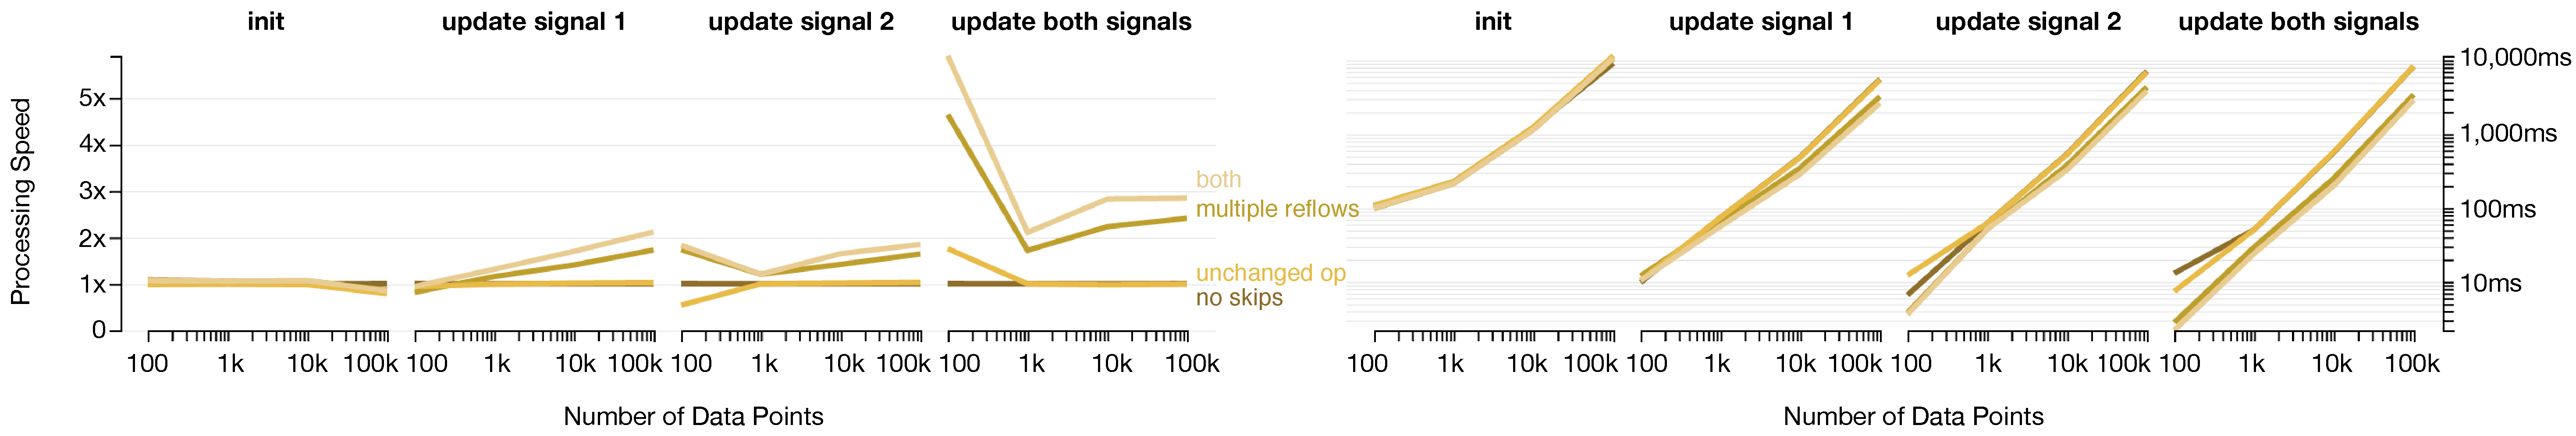
\includegraphics[width=\columnwidth]{skips-lines.pdf}
  \caption{The effects of pruning unnecessary computation on average processing
speed. (a) A relative difference between conditions (higher is better). (b)
Absolute values for time taken, plotted on a log$_{10}$ scale (lower is better).}
  \label{fig:vg:skips_benchmark}
\end{figure}

By centralizing responsibility for operator scheduling and changeset dispatch,
we can aggressively prune unnecessary recomputation. The dataflow graph
scheduler knows the current state of the propagation, and dependency
requirements for each queued operator, allowing us to perform two types of
optimizations:

\begin{enumerate}
  \item \emph{Pruning multiple reflows of the same branch}. As the scheduler
  ensures a topological propagation ordering, a branch can be safely pruned for
  the current propagation if it has already been reflowed.

  \item \emph{Skipping unchanged operators}. Operators identify their
dependencies\,---\,including signals, data fields, and scale functions\,---\,and
changesets maintain a tally of updated dependencies as they flow through the
graph. The scheduler skips evaluation of an individual operator if it is not
responsible for deriving new tuples, or if a changeset contains only modified
tuples and no dependencies have been updated. Downstream operators are still
queued for propagation.
\end{enumerate}

To measure the impact of these optimizations, we created a grouped bar chart
with five data transformation operators: \texttt{Derive(signal1)} $\rightarrow$
\texttt{Fold} $\rightarrow$ \texttt{Derive(signal2)} $\rightarrow$
\texttt{Filter (signal2)} $\rightarrow$ \texttt{Facet}.  We then benchmarked the
effect of four conditions (processing all recomputations, pruning multiple
reflows only, skipping unchanged operators only, and applying both
optimizations) across four tasks (initializing the visualization, updating each
signal in turn, and updating both signals together).

Results are shown in Figure~\ref{fig:vg:skips_benchmark}. Preventing multiple
reflows is the most effective strategy, increasing throughput 1.4 times on
average. Skipping unchanged operators sees little benefit by itself as, in our
benchmark setup, only the two operators following a fold are skipped when
changing \texttt{signal1}, and only the first derivation operator is skipped
when changing \texttt{signal2}. When the two strategies are combined, however,
we see a 1.6x increase in performance. This result was consistent across
multiple benchmark trials. After careful hand-verification to ensure no
additional nodes were erroneously skipped, we hypothesize that the JavaScript
runtime is able to perform just-in-time optimizations that it is unable to apply
to the other conditions.

\subsection{Inlining Sequential Operators}

\begin{figure}[h!]
  \centering
  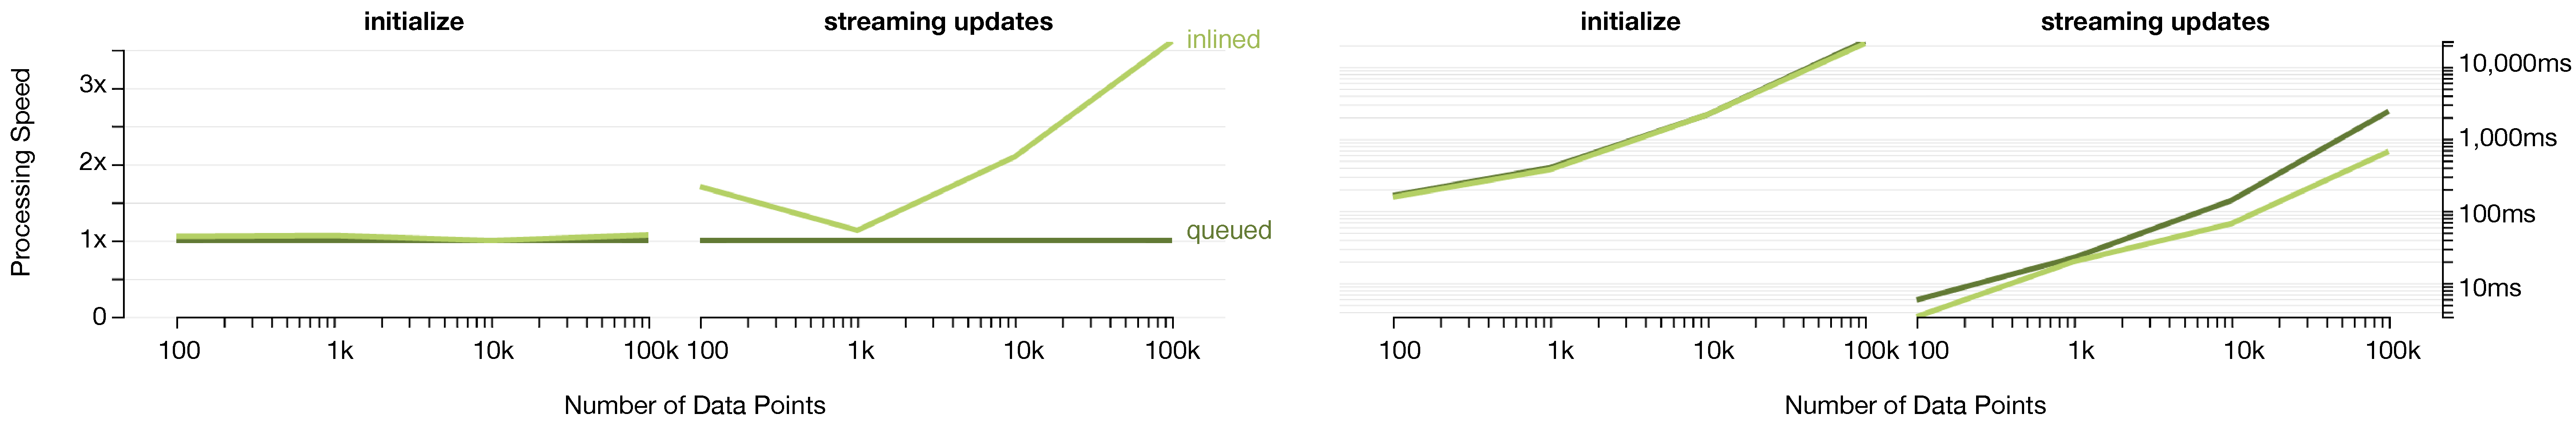
\includegraphics[width=\columnwidth]{inlined-lines.pdf}
  \caption{The effects of inlining sequential operators on average processing
speed. (a) A relative difference between conditions (higher is better). (b)
Absolute values for time taken, plotted on a log$_{10}$ scale (lower is better).}
  \label{fig:vg:inline_benchmark}
\end{figure}

To propagate changesets through the dataflow graph, the scheduler adds operators
to a priority queue, backed by a binary heap sorted in topological order. This
incurs an $O(log N)$ cost for enqueueing and dequeueing operators, which can be
assessed multiple times per operator if the graph is dynamically restructured.
However, branching only occurs when operators register dependencies, and
dependencies are only connected to \texttt{Collector} nodes. As a result, much
of the dataflow graph comprises linear paths. This is particularly true for
scene graph operators, which are grouped into hundreds (or even thousands) of
independent mark build-evaluate-bound branches.

We explore the effect of inline evaluation of linear branches, whereby operators
indicate that their neighbors can be called directly rather than queued for
evaluation. The scheduler remains responsible for propagating the changeset,
and thus can continue to apply the optimizations previously discussed. Although
inline evaluation can be applied in a general fashion by coalescing linear
branches into ``super nodes,'' for simplicity we only evaluate inlining of scene
graph operators here. Mark builders directly call evaluators and bounders, and
group mark builders directly call new child mark builders rather than forming a
temporary connection.

Figure~\ref{fig:vg:inline_benchmark} shows the results of this optimization
applied to a parallel coordinates plot. The plot uses a nested scene graph in
which each line segment is built by a dedicated build-evaluate-bound branch. As
we can see, inlining does not have much impact on the initialization time. This
is unsurprising, as the largest initialization cost is due to unavoidable graph
restructuring. However, inlining improves streaming operations by a 1.9x factor
on average. As streaming updates only propagate down specific branches of the
dataflow graph, inline evaluation results in at least 4 fewer queuing operations
by the scheduler.
% !TEX root = ../thesis.tex

\vspace{-20pt}

\section{Comparative Performance Benchmarks}
\label{sec:vg:performance}

\vspace{-10pt}

To evaluate the performance of Reactive Vega against D3~\cite{bostock:d3} and
the origin, non-reactive Vega system (v1.5.0), we use the same setup described
in the previous section.

\vspace{-10pt}

\subsection{Streaming Visualizations}

\vspace{-7pt}

Figure~\ref{fig:vg:static_benchmark} shows the average performance of
uninteractive streaming scatter plots, parallel coordinates plots, and trellis
plots. We first measured the average time to initially parse and render the
visualizations. To gauge streaming performance, we next measured the average
time taken to update and re-render upon adding, modifying, or removing 1\% of
tuples. We ran 10 trials per dataset, sized 100--100,000 tuples.

\begin{figure}[t!]
  \centering
  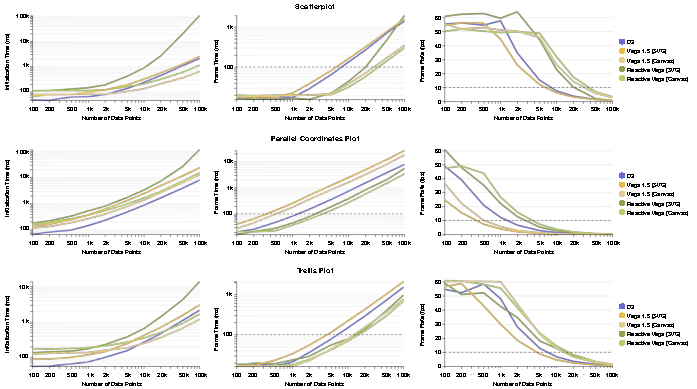
\includegraphics[width=\columnwidth]{streaming-lines.pdf}
  \caption{Average performance of rendering (non-interactive) streaming visualizations:
(top-bottom) scatterplot, parallel coordinates, and trellis plot; (left-right)
initialization time, average frame time, and average frame rate. Dashed lines
indicate the threshold of interactive updates~\cite{card:modelhuman}.}
  \label{fig:vg:static_benchmark}
\end{figure}

Reactive Vega has the greatest effect with the parallel coordinates plot,
displaying 2x and 4x performance increases over D3 and Vega 1.5, respectively.
This effect is due to each plotted line being built and encoded by its own
dataflow branch. Across the other two examples, and averaging between the Canvas
and SVG renderers, we find that although Reactive Vega takes 1.7x longer to
initialize the visualizations, subsequent streaming operations are 1.9x faster
than D3. Against Vega 1.5, Reactive Vega is again 1.7x slower at initializing
visualizations; streaming updates perform roughly op-par with the Canvas
renderer, but are 2x faster with the SVG renderer.

Slower initialization times for Reactive Vega are to be expected. D3 does not
have to parse and compile a JSON specification, and a streaming dataflow graph
is a more complex execution model, with higher overheads, than batch processing.
However, with streaming visualizations this cost amortizes and performance in
response to data changes becomes more important. In this case, Reactive Vega
makes up the difference in a single cycle.

\vspace{-10pt}

\subsection{Interactive Visualizations}

\vspace{-7pt}

We evaluated the performance of interactive visualizations (measured in terms of
interactive frame rate) using three common examples: brushing \& linking a
scatterplot matrix, a time-series overview+detail visualization, and panning \&
zooming a scatterplot. We chose these examples as they all leverage interactive
behaviors supported by D3, with canonical implementations available for
each\footnote{Brushing \& Linking:
http://bl.ocks.org/mbostock/4063663}\textsuperscript{,}\footnote{Overview +
Detail: http://bl.ocks.org/mbostock/1667367}\textsuperscript{,}\footnote{Pan \&
Zoom: http://bl.ocks.org/mbostock/3892919}. For Reactive Vega, we expressed
these visualizations with a single declarative specification. For D3 and Vega
1.5, we use custom event handling callbacks. The Vega 1.5 callbacks mimic the
behavior of the fragmented reactive approach used in prior
work~\cite{satyanarayan:declarative}. We tested these visualizations with
datasets sized between 100 and 10,000 tuples.

\begin{figure}[t!]
  \centering
  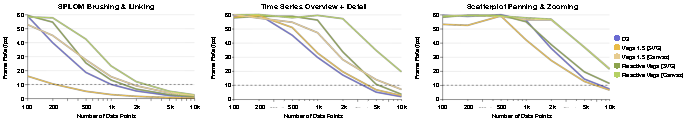
\includegraphics[width=\columnwidth]{interaction-lines.pdf}
  \caption{Average frame rates for three interactive visualizations: (left-right)
  brushing and linking on a scatterplot matrix; brushing and linking on an
  overview+detail visualization; panning and zooming on a scatterplot. Dashed
  lines indicate the threshold of interactive updates~\cite{card:modelhuman}.}
  \label{fig:vg:interactive_benchmark}
\end{figure}

Figure~\ref{fig:vg:interactive_benchmark} shows the results\,---\,on average,
and across both Canvas and SVG renderers, Reactive Vega offers superior
interactive performance to custom D3 and Vega event handling callbacks. This
effect primarily stems from Reactive Vega's unified data model, and is most
noticeable with brushing \& linking a scatterplot matrix and the time-series
overview+detail visualization. In both examples, interactions manipulate only a
subset of all data tuples. With Reactive Vega, only these tuples are processed,
and their corresponding scene graph elements re-encoded and re-rendered. In
contrast, Vega 1.5's fragmented reactive approach reconstructs and re-renders
the entire scene graph in response to changing data.
% !TEX root = ../thesis.tex
\section{Conclusion \& Future Work}
\label{sec:vg:conclusion}

Declarative languages are a popular means of authoring
visualizations~\cite{bostock:protovis, bostock:d3, heer:protovisjava}, but have
lacked first-class support for interaction design. In response, we contribute
Reactive Vega, the first language and system architecture to support declarative
visualization and interaction design in a comprehensive and performant fashion.

It is important to note that although Reactive Vega provides an complete
end\--to\--end system\,---\,whereby users invoke the parser to traverse an
input declarative specification and instantiate the necessary architecture
components to render a visualization\,---\,this process can be decoupled.
Reactive Vega's declarative model can be used to implement extensions to D3, and
higher-level tools can opt to manually construct and connect required dataflow
operators.

By simplifying programmatic generation of visualization, Reactive Vega's
declarative JSON syntax has led to a growing ecosystem of higher-level
visualization systems. For example, MapD~\cite{mapd:vega} has integrated Vega
with their GPU-powered database; custom SQL queries can be embedded within the
JSON specification, which is dispatched to the backend server, rendered, and
returned to the client as a PNG image. Similarly, Wikipedia, a security-concious
environment where it would be difficult to allow users to write imperative
visualization code, has recently integrated Vega~\cite{mediawiki:graph} to
enable visualization of data embedded in articles.

Still, improved support for authoring and debugging Vega specifications remains
a promising avenue for future work. In recent work, Hoffswell
et~al.~\cite{hoffswell:debugging} developed a ``time-traveling'' debugger for
Reactive Vega specifications and found that first-time Vega users were able to
accurately trace errors through the specification. Further work, particularly by
instrumenting Reactive Vega's dataflow graph to enable inspection and stepping
through changeset propagation could aid in learnability~\cite{guo:tutor}.
Through the development of such tools, we can also assess the accessibility of
the language. Are new users able to learn the declarative interaction model? Can
experts, accustomed to callback-driven programming, quickly transition as well?

Reactive Vega's architecture also offers opportunities to study scalable
visualization design. Interactive visualization of large-scale datasets often
requires offloading computation to server-side architectures. For example,
Nanocubes~\cite{lins:nanocubes} and imMens~\cite{liu:immens} assemble
multi\--dimensional data cubes that can be decomposed into smaller data tiles
and pushed to the client. Such components could be integrated into a dataflow
graph with execution distributed across server and client~\cite{domoritz:dsia}.
For example, as the dataflow graph scheduler is responsible for propagation, it
might anticipate possible user interactions and prefetch data tiles in order to
reduce latency~\cite{battle:prefetch}.

Reactive Vega is an open source system available at
\url{http://vega.github.io/vega/}.